% !TEX program = xelatex
\documentclass[a4paper]{article}
\usepackage[UTF8]{ctex}
\setCJKmainfont{SimSun}[BoldFont=SimHei,ItalicFont=KaiTi]
\setCJKsansfont{SimHei}
\usepackage[top=2mm,bottom=2mm,left=2mm,right=2mm]{geometry}
\usepackage{amsmath,amssymb,bm}
\usepackage{multicol}
\usepackage{tabularx,array}
\usepackage{graphicx}
\usepackage{tikz}
\usetikzlibrary{arrows.meta,calc}
\usepackage[dvipsnames]{xcolor}
\pagestyle{empty}
\setlength{\parindent}{0pt}
\setlength{\parskip}{0pt}
\setlength{\columnsep}{1.35mm}
\setlength{\columnseprule}{0.12pt}
\setlength{\tabcolsep}{0.8pt}
\setlength{\fboxsep}{0.45pt}
\renewcommand{\baselinestretch}{0.58}
\definecolor{h}{HTML}{0B3D91}
\definecolor{b}{HTML}{1565C0}
\definecolor{o}{HTML}{E65100}
\definecolor{r}{HTML}{B71C1C}
\definecolor{g}{HTML}{1B5E20}
\definecolor{bg}{HTML}{EEF3FF}
\definecolor{warnbg}{HTML}{FFF2E6}
\definecolor{grid}{HTML}{D6DEE8}
\newsavebox{\fitbox}
\newcommand{\fitmath}[2][\dimexpr\linewidth-4pt\relax]{\sbox{\fitbox}{$\displaystyle #2$}\ifdim\wd\fitbox>#1\resizebox{#1}{!}{$\displaystyle #2$}\else\usebox{\fitbox}\fi}
\newcommand{\HH}[1]{\vspace{0.25pt}{\fontsize{5.45}{5.60}\selectfont\bfseries\color{white}\colorbox{h}{\strut\ #1\ }}\par\vspace{0.15pt}}
\newcommand{\K}[1]{\textbf{\color{b}#1}}
\newcommand{\R}[1]{\textbf{\color{r}#1}}
\newcommand{\OO}[1]{\textbf{\color{o}#1}}
\newcommand{\G}[1]{\textbf{\color{g}#1}}
\newcommand{\F}[1]{\colorbox{bg}{\fitmath{#1}}}
\newcommand{\card}[2]{\vspace{0.16pt}\noindent\fcolorbox{grid}{white}{\begin{minipage}{0.982\linewidth}\fontsize{4.16}{4.34}\selectfont\textbf{\color{h}#1}\par #2\end{minipage}}\par}
\newcommand{\tree}[5]{\card{#1}{\K{识别}：#2\par\K{第一行}：#3\par\K{主链}：#4\par\K{子集}：#5}}
\newcommand{\sub}[3]{\OO{#1}｜#2\quad\K{链}：#3\par}
\newcommand{\chk}[1]{\colorbox{warnbg}{\begin{minipage}{\dimexpr\linewidth-2\fboxsep\relax}\fontsize{4.05}{4.22}\selectfont\R{检查}：#1\end{minipage}}\par}
\newcommand{\tinyfig}[1]{\begin{center}\vspace{-1pt}#1\vspace{-4pt}\end{center}}
\newcommand{\pipefig}{\tinyfig{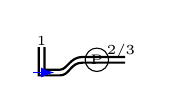
\begin{tikzpicture}[>=Latex,scale=.36,every node/.style={font=\tiny}]
\draw[thick](0,1)--(0,0)--(.75,0)..controls(1.1,0)and(1.1,.45)..(1.55,.45)--(3.05,.45);
\draw[thick](.2,1)--(.2,.2)--(.75,.2)..controls(1.0,.2)and(1.1,.65)..(1.55,.65)--(3.05,.65);
\draw[->,blue](-.2,.1)--(.55,.1);\node[circle,draw,inner sep=1pt] at (2.05,.55){P};\node at(.1,1.2){1};\node at(2.9,.85){2/3};
\end{tikzpicture}}}
\newcommand{\hydrofig}{\tinyfig{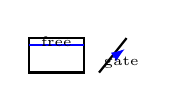
\begin{tikzpicture}[>=Latex,scale=.35,every node/.style={font=\tiny}]
\draw[thick](0,0)--(2,0)--(2,1.25)--(0,1.25)--cycle;\draw[blue](0,1)--(2,1);\draw[thick](2.55,0)--(3.55,1.25);
\draw[->,blue](3.05,.55)--(3.48,.85);\node at(1,1.12){free};\node at(3.35,.35){gate};
\end{tikzpicture}}}
\newcommand{\cvfig}{\tinyfig{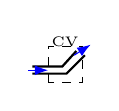
\begin{tikzpicture}[>=Latex,scale=.36,every node/.style={font=\tiny}]
\draw[thick](0,.3)--(1.2,.3)--(1.85,.95);\draw[thick](0,.55)--(1.05,.55)--(1.55,1.1);\draw[dashed](.55,.0)rectangle(1.75,1.25);
\draw[->,blue](-.15,.42)--(.55,.42);\draw[->,blue](1.47,.95)--(2.05,1.32);\node at(1.15,1.43){CV};
\end{tikzpicture}}}
\newcommand{\potfig}{\tinyfig{\begin{tikzpicture}[>=Latex,scale=.34,every node/.style={font=\tiny}]
\foreach \y in{-.35,0,.35}{\draw[->,blue](-.1,\y)--(.8,\y);}\draw[thick](1.15,0)circle(.32);\node at(1.15,-.55){cyl};
\draw[fill=black](2.1,0)circle(.04);\node[above]at(2.1,0){源};\draw[thick](2.75,-.5)..controls(3.2,-.75)and(3.6,-.75)..(4.0,-.5);
\end{tikzpicture}}}
\newcommand{\lavalfig}{\tinyfig{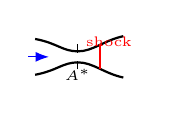
\begin{tikzpicture}[>=Latex,scale=.35,every node/.style={font=\tiny}]
\draw[thick](0,.65)..controls(.8,.5)and(1.0,.2)..(1.55,.2)..controls(2.1,.2)and(2.5,.6)..(3.2,.75);
\draw[thick](0,-.65)..controls(.8,-.5)and(1.0,-.2)..(1.55,-.2)..controls(2.1,-.2)and(2.5,-.6)..(3.2,-.75);
\draw[dashed](1.55,-.45)--(1.55,.45);\node at(1.55,-.65){$A^*$};\draw[->,blue](-.25,0)--(.5,0);\draw[red,thick](2.35,-.45)--(2.35,.45);\node[red]at(2.68,.55){shock};
\end{tikzpicture}}}
\newcommand{\blfig}{\tinyfig{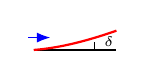
\begin{tikzpicture}[>=Latex,scale=.35,every node/.style={font=\tiny}]
\draw[thick](0,0)--(3.0,0);\draw[->,blue](-.2,.45)--(.6,.45);\draw[red,thick](0,0)..controls(1,.08)and(2,.35)..(3,.7);\draw[dashed](2.2,0)--(2.2,.55);\node[right]at(2.2,.3){$\delta$};
\end{tikzpicture}}}
\begin{document}
\fontsize{4.23}{4.42}\selectfont

% ================= PAGE 1 =================
\begin{multicols}{3}
\HH{P1 总入口 + 母题A：管路/泵/水轮机/汽蚀}
\card{先别翻公式：每题先选母题树}{A 管路能量：水池、长管、泵、阀、压力表、汽蚀、水轮机。\par
B 静水：静止液体、U管、闸门、浮体、曲面受压。\par
C 动量：弯管、喷流、喷嘴、叶片、支座力。\par
D 势流：源汇涡、镜像、圆柱、环量、机翼。\par
E 可压：$Ma,p_0,T_0,A^*,p_b$、喷管、激波、膨胀角。\par
F 粘性/阻力：$Re,\mu,\tau_w,\delta,C_D$、Moody、边界层。\par
G 代数概念：速度场、应力张量、量纲、证明。}
\card{每题第一行模板}{取\_\_为研究对象，设1为\_\_，2为\_\_，取\_\_为正，在\_\_假设下列\_\_方程。最后补：单位、方向、表压/绝压、查表入口。}
\F{Q=AV,\quad \dot m=\rho Q,\quad Re=VL/\nu=\rho VL/\mu,\quad Ma=V/\sqrt{\gamma RT}}
\pipefig
\tree{母题A总树：管路机械能}{水池/管路/泵/水轮机/弯头阀门/压力表/粗糙度/汽蚀}{取1上游已知能量处，2目标截面，3出口或机器后；液面/自由射流常取表压0}{几何$A,L,d,z\to V_i=Q/A_i\to Re_i\to \lambda_i\to h_f,h_\zeta\to$修正Bernoulli}{\sub{求$Q$}{水位差/出口大气}{把$V_i=Q/A_i$，损失写成$KQ^2$；若$\lambda(Re)$未知则试算迭代}\sub{求$p$}{压力表/某截面压强}{已知$Q$先算全部损失，从已知压强截面列到未知截面}\sub{求泵/水轮机功率}{扬程/效率/输出功率}{先由能量式求$H_p$或$H_T$；泵轴功率除$\eta$，水轮机输出乘$\eta$}\sub{求汽蚀安装高度}{汽化压/入口压至少高于}{水面到泵入口列能量，令$p_{in}\ge p_v+\Delta p$，全用绝压}}
\card{A母公式：水头式}{\F{z_1+\frac{p_1}{\rho g}+\frac{\alpha_1V_1^2}{2g}+H_p=z_2+\frac{p_2}{\rho g}+\frac{\alpha_2V_2^2}{2g}+H_T+h_f+h_\zeta}\par
\F{h_f=\sum\lambda_i\frac{L_i}{d_i}\frac{V_i^2}{2g},\quad h_\zeta=\sum\zeta_j\frac{V_j^2}{2g}}\par
\F{P_{\rm pump,shaft}=\rho gQH_p/\eta,\quad P_T=\eta\rho gQH_T}}
\card{A子集：求流量$Q$}{\K{触发}：水池接长管/出口到大气/问流量。\par
\K{落笔}：1水面，2出口；$p_1=p_2=0$表压，$V_1\approx0$。\par
\K{链}：$H=z_1-z_2=(1+\lambda L/d+\sum\zeta)V^2/(2g)$，$Q=AV$。\par
\K{变形}：多管径则每段$V_i=Q/A_i$；并联不是损失相加，而是$h_{La}=h_{Lb}$，$Q=Q_a+Q_b$。}
\card{A子集：求压力/压力表}{\K{触发}：给$Q$、压力表、某点压强。\par
\K{链}：$Q\to V_i\to Re_i\to \lambda_i\to h_L$；从已知点到未知点移项解$p$。\par
\K{表压}：水池自由面/大气出口表压0；真空表为负表压；气体/汽蚀换绝压。\par
\K{位置}：压力表接在管中心线；若题强调管顶/管底，补竖向高度差。}
\card{A子集：汽蚀/最大安装高度}{\K{触发}：离心泵吸水、汽化压、入口压至少高于汽化压20kPa。\par
\K{第一行}：从吸入水面1到泵入口2列能量。\par
\K{链}：$p_2=p_a-\rho gh-\frac12\rho V^2-\rho gh_{L,12}$；令$p_2\ge p_v+\Delta p$，解$h_{\max}$。\par
\K{查表}：吸入管有粗糙度/弯头/阀门，先算$Re,\epsilon/d\to\lambda,\zeta$。}
\card{A子集：泵/水轮机/效率}{\K{泵}：给流体加能，方程左边$+H_p$；若题给轴功率，$H_p=\eta P_s/(\rho gQ)$。\par
\K{水轮机}：从流体取能，输出轴功率$P_s=\eta\rho gQH_T$；若问水流失去功率，不乘效率。\par
\K{反制}：kW不能直接当压强；$m^3/h$先除3600。}
\card{A子集：粗糙/串并联/局部件}{\K{粗糙}：题干有铸铁/镀锌/粗糙度$e$，先$e/d$，再和$Re$查Moody；层流$\lambda=64/Re$不用查。\par
\K{串联}：同$Q$，不同$d$导致不同$V_i,Re_i$，损失逐段加。\par
\K{并联}：同端点水头差相等，$h_{La}=h_{Lb}$，且$Q=Q_a+Q_b$。\par
\K{局部}：阀/弯头/入口用所在管段速度头；突然扩大优先$(V_1-V_2)^2/(2g)$。}
\card{A答题收口}{故$Q=\_\_\,m^3/s$，或$p=\_\_\,kPa$（表压/绝压），或$P=\_\_\,kW$（轴功率/水功率）。损失项非负；若泵扬程算负，通常是方向或机器类型设反。}
\card{A子集树：题干图形怎么归入能量题}{\K{两大水池+长管}：$p_1=p_2=0$表压，$V_1,V_2\approx0$，高差全变损失/出口速度。\par
\K{泵在管中}：泵前后各取一截面，泵给流体加$H_p$；题问轴功率再除效率。\par
\K{水轮机在管中}：水轮机从流体取$H_T$；题问输出功率乘效率。\par
\K{虹吸/吸水管}：最低压常在高点或泵入口；必须用绝压和汽化压检查。\par
\K{压力表/真空表}：表压直接进$p/\rho g$；真空表读数是负表压。}
\card{A子集树：未知量反推顺序}{\K{已知$Q$求$p$}：先$V_i$，再$Re_i$，再$\lambda_i,\zeta_i$，最后能量式移项。\par
\K{已知$p$求$Q$}：把$h_L=K(Q)Q^2$；若$\lambda$未知，先假设$\lambda$，解$Q$，重算$Re$查$\lambda$，迭代到变化小。\par
\K{已知泵功率求$Q$}：$H_p=\eta P_s/(\rho gQ)$含$Q$，代入能量式形成关于$Q$的方程。\par
\K{并联分流}：不能先平均分流；先写各支路同水头损失，再加总流量。}
\card{A子集树：局部损失和速度头}{入口、出口、阀门、弯头、突然扩大/缩小都归入$h_\zeta=\zeta V^2/(2g)$。\par
若局部件前后管径不同，题目没特殊说明时用该局部件所在管段速度；突然扩大常用$(V_1-V_2)^2/(2g)$。\par
出口到大气的速度头不要凭空丢掉：若截面2取在自由射流，保留$V_2^2/2g$；若取在下游大水池液面，速度约0但中间有出口损失。}
\card{A子集树：能量线/压强线题}{总水头线EGL：$z+p/\rho g+\alpha V^2/(2g)$；测压管水头线HGL：$z+p/\rho g$。\par
沿程损失让两条线下降；泵使EGL/HGL跳升；水轮机使其跳降；管径变小速度头变大，HGL可突然下降。\par
若问“哪里易汽蚀”，找HGL最低且绝压接近汽化压的位置。}
\card{A子集树：管路考试最常见外壳}{\K{求安装高度}：水面$\to$泵入口，约束$p_{\rm in}/\rho g\ge p_v/\rho g+\Delta h_{\rm safe}$。\par
\K{求水轮机输出}：上游水面$\to$下游水面，$H_T=$可取出的能量；$P=\eta\rho gQH_T$。\par
\K{求某表压}：从自由液面或已知表压点列到表点，注意表点高程。\par
\K{求管径}：$Q$已知则$V=4Q/\pi d^2$，$Re,\lambda,h_f$都含$d$，通常试算。}
\card{A子集树：文丘里/孔口/喷嘴流量计}{\K{触发}：压差计、喉部、孔板、喷嘴、流量系数。\par
\K{理想链}：连续$Q=A_1V_1=A_2V_2$，Bernoulli给$p_1-p_2=\frac12\rho(V_2^2-V_1^2)$。\par
\K{实际链}：乘流量系数$C_d$，$Q=C_dA_2\sqrt{\frac{2\Delta p/\rho}{1-(A_2/A_1)^2}}$。\par
\K{压差计}：$\Delta p=(\rho_m-\rho)gh$常见；若两端高度不同，先按静水逐段修正。}
\card{A子集树：虹吸管/负压高点}{虹吸题先从上游水面到管顶最高点列能量：$p_{\rm top}/\rho g=z_1-z_{\rm top}-V^2/2g-h_{L,1\to top}$。\par
约束$p_{\rm top}\ge p_v$；若题给“避免汽蚀/断流”，还要留安全余量。\par
再从上游水面到出口列能量求$Q$。最高点不一定控制流量，但控制能否工作。}
\card{A子集树：泵串并联和管路特性}{单泵特性若给$H_p(Q)$，系统曲线为$H_{\rm need}=H_0+KQ^2$。\par
串联泵：同流量扬程相加；并联泵：同扬程流量相加。\par
若题只给一台泵功率，不要直接把功率相加成水头；先换$H_p=\eta P/(\rho gQ)$。}
\card{A子集树：单位和数量级保底}{$1\,Pa=1\,N/m^2$，$p/\rho g$单位m；$1\,kPa\approx0.102m$水头，$1m$水头$\approx9.81kPa$。\par
$d$用m，面积$\pi d^2/4$；$Q=50m^3/h=0.0139m^3/s$。\par
水管平均速度常在$0.5\sim5m/s$量级；若算出几十上百$m/s$，检查面积/单位。}
\card{A子集树：完整落笔模板}{“取上游自由液面1和目标截面2，沿流向列修正Bernoulli：\par
$z_1+p_1/\rho g+\alpha_1V_1^2/2g+H_p=z_2+p_2/\rho g+\alpha_2V_2^2/2g+H_T+\sum h_L$。\par
其中$V_i=Q/A_i$，$Re_i=V_id_i/\nu$，由$Re_i,e/d_i$取$\lambda_i$，局部损失按题给$\zeta$计。最后解\_\_并检查表压/绝压。”}
\chk{水头式每项单位都是m；不要把Pa直接和m相加。自由面速度约0只在大水池成立。出口自由射流要保留出口速度头。}
\end{multicols}
\newpage

% ================= PAGE 2 =================
\begin{multicols}{3}
\HH{P2 母题B/C/D：静水 + CV动量 + 势流}
\hydrofig
\tree{母题B总树：静水压强与受力}{静止液体/U管/闸门/曲面/浮体/测压管}{流体静止，压强只随竖直深度变化；先写$p=p_0+\rho gh$}{点压强$\to$受压面积形心$\to$合力$\to$作用点/分量$\to$力矩或稳定}{\sub{点压强/U管}{多液体/水银/差压}{沿液柱走：向下加$\rho gh$，向上减；同一静止连通液体同高等压}\sub{平面闸门}{矩形/圆形/倾斜/铰链}{形心深度求合力，压力中心求力臂，再对铰链取矩}\sub{曲面挡水}{圆弧门/曲面}{水平分量用竖直投影，竖直分量用假想水体重量}\sub{浮力稳定}{漂浮/沉没/排水体积}{浮力=排开液体重，漂浮$F_B=G$}}
\card{B公式链}{\F{p=p_0+\rho gh,\quad F=\rho gh_cA,\quad h_p=h_c+\frac{I_G}{h_cA}}\par
倾斜面：$h=s\sin\theta$，沿板坐标可写$s_p=s_c+I_G/(s_cA)$。\par
曲面：$F_H=$竖直投影面静水压力，$F_V=$曲面上方/下方假想液体重量，$R=\sqrt{F_H^2+F_V^2}$。\par
浮力：$F_B=\rho_f gV_{\rm disp}$。}
\card{B子集：U管/测压}{\K{触发}：U形管、水银、油水、多液体、压差。\par
\K{链}：从已知压强端出发，沿液柱逐段加减$\rho gh$；同一水平同种连通液体压强相等。\par
\K{错}：不能把水银高度直接当水头；两端若是气体，液面上方气压要保留。}
\card{B子集：闸门/铰链}{\K{触发}：矩形板、圆板、倾斜门、拉力、铰链。\par
\K{链}：$h_c\to F\to h_p/s_p\to$对铰链取矩。\par
\K{错}：合力大小用形心深度，合力作用点是压力中心；压力中心比形心更深。}
\card{B子集：曲面/浮体}{\K{曲面}：别用曲面面积乘形心压强；先$F_H$、再$F_V$、最后合成方向。\par
\K{浮体}：只判上浮/下沉可比平均密度；终速题还要写重力-浮力-阻力=0。}
\card{B子集树：静水题外壳合并}{\K{开口容器}：自由面$p=p_a$；用表压时自由面为0。\par
\K{密闭容器}：液面上方气压不能丢，先写$p_{\rm surface}$再加$\rho gh$。\par
\K{多液体}：不要合并密度；每一段液柱单独$\rho_i g\Delta h_i$。\par
\K{倾斜板}：深度是竖直深度$h$，不是板长$s$；只有换压力中心坐标时才用$s=h/\sin\theta$。}
\card{B子集树：受力方向和力矩}{平面受压合力垂直板面，方向由水压推板；曲面合力方向由$F_H,F_V$合成。\par
铰链题：先设未知拉力/支反力方向，再对铰链取矩消掉支反力。若题问最小拉力，通常让拉力力臂最大或刚好临界开启。\par
浮体稳定：只需静态平衡时写$G=F_B$；若问倾覆稳定，比较重心、浮心、稳心位置。}
\cvfig
\tree{母题C总树：控制体动量反力}{弯管、喷嘴、水枪、射流打板、叶片、支座反力}{取流体为CV，画$x,y$正方向，先假设外界对流体反力}{连续/能量求$V,p\to$列压力力/重力/支座力$\to\sum F=\dot m(V_2-V_1)\to$按题问对象取反}{\sub{弯管支座}{管流转弯/支承力}{压力力压入截面，重力若竖直弯管不可漏，最后管受力取反}\sub{喷流打板}{自由射流/偏转角}{自由射流表压0，理想光滑板速度大小不变，只变方向}\sub{喷嘴水枪}{渐缩喷嘴/握持力}{先能量求出口速度和入口压强，再动量求反力}\sub{叶轮功率}{半径/角速度/切向速度}{只取切向动量矩，$M=\dot m(r_2V_{u2}-r_1V_{u1})$}}
\card{C公式链}{\F{\sum F_x=\dot m(V_{2x}-V_{1x}),\quad \sum F_y=\dot m(V_{2y}-V_{1y})}\par
\F{\dot m=\rho Q,\quad M_z=\dot m(r_2V_{u2}-r_1V_{u1}),\quad P=M\omega}\par
压力力按截面法向压入CV；自由射流/大气出口表压0。}
\card{C子集：弯管/喷嘴/板}{\K{弯管}：设支座对流体$R_x,R_y$，列两方向动量；题问“流体对管”就整体取负。\par
\K{喷嘴}：入口压力常不能省；出口大气表压0。\par
\K{板}：固定光滑板近似$|V_2|=|V_1|$，只投影方向。}
\card{C子集树：动量题外壳合并}{\K{弯管支座}：先由能量/连续求$V,p$，再进动量；压力力方向沿截面法线压入CV。\par
\K{消防水枪/喷嘴}：自由出口$p_2=0$表压；入口$p_1A_1$不能漏。\par
\K{射流冲板}：若板固定，流量$\dot m=\rho Q$；若板运动，相对流量用$\rho A(V-U)$。\par
\K{叶片/叶轮}：力用线动量，功率用角动量；只取切向分量做功。}
\card{C子集树：对象取反规则}{动量方程求的是“外界对控制体内流体的合力”。\par
题问管壁/板/喷嘴受到的力：最后取反。\par
支座反力与流体对固体力也相反；若求螺栓/支座需要承担的力，通常等于固定该固体所需的外力。}
\potfig
\tree{母题D总树：势流叠加}{无旋、不可压、势函数、流函数、源汇涡、镜像、圆柱、环量}{先写基本流$\varphi,\psi$并线性叠加；固壁为$\psi=C$或$v_n=0$}{总$\varphi/\psi\to$速度分量$\to$驻点/边界$\to$Bernoulli压强或环量升力}{\sub{基本流}{均匀流/源汇/点涡/偶极}{背表：源给径向流量，涡给环量；复杂题先叠加}\sub{镜像壁面}{直壁/不可穿透}{源靠壁同号，涡靠壁反号，目的是抵消法向速度}\sub{圆柱环量}{圆柱/机翼/升力}{表面$r=a$，先$v_\theta$，再$C_p$和$L'$}\sub{非定常势流}{U管振荡/加速势流}{普通定常Bernoulli不够，要加$\partial\varphi/\partial t$}}
\card{D公式链}{直角：$u=\varphi_x=\psi_y,\ v=\varphi_y=-\psi_x$；极坐标：$v_r=\varphi_r=\frac1r\psi_\theta,\ v_\theta=\frac1r\varphi_\theta=-\psi_r$。\par
均匀流：$\varphi=Ur\cos\theta,\psi=Ur\sin\theta$；源：$\varphi=\frac{Q}{2\pi}\ln r,\psi=\frac{Q}{2\pi}\theta$；涡：$v_\theta=\Gamma/(2\pi r)$。}
\card{D子集：圆柱/机翼/压力}{圆柱表面无环量：$v_\theta=-2U\sin\theta$，$C_p=1-4\sin^2\theta$。\par
有环量：$v_\theta=-2U\sin\theta+\Gamma/(2\pi a)$，$L'=\rho U\Gamma$。\par
势流压力：$p=p_\infty+\frac12\rho(U_\infty^2-V^2)$。速度越大，压强越小。}
\card{D子集树：基本流表要怎么用}{\K{均匀流}：给远处来流，直接写$\varphi=Ur\cos\theta,\psi=Ur\sin\theta$。\par
\K{源/汇}：给流量$Q$或半体，源为$+Q$、汇为$-Q$；驻点由总速度为0求。\par
\K{点涡}：给环量$\Gamma$或升力；涡只给切向速度，除原点外无旋。\par
\K{偶极}：圆柱绕流本质是均匀流+偶极；不必每次重新解Laplace。}
\card{D子集树：镜像和边界}{直固壁要$v_n=0$，即壁面是一条流线$\psi=C$。\par
源靠固壁：放同号镜像；点涡靠固壁：放反号镜像。两个壁面时连续镜像，或按角域基本解。\par
若壁面是对称面，只保留半平面流量：例如半平面源/汇分母可从$2\pi$变成$\pi$。}
\card{D子集树：势流题收口}{求压力先求速度；求力先求压力分布再积分，或直接用已知升力定理。\par
圆柱无环量阻力为0是理想势流结论；有环量有升力$L'=\rho U\Gamma$，方向由环量和来流右手判定。\par
非定常势流/U管振荡必须用$\partial\varphi/\partial t$项，不能只用定常Bernoulli。}
\card{B子集树：常见静水图形模板}{\K{矩形闸门}：$A=bh_c$不对；应为$A=bs$或$bH$，$h_c$只用于压强。\par
\K{圆形闸门}：$A=\pi R^2$，$I_G=\pi R^4/4$；若板倾斜，深度用$h_c$，沿板位置用$s_p$。\par
\K{圆弧门}：$F_H$等于竖直投影受力，$F_V$等于曲面上方假想液体重量；方向看假想水体在曲面哪侧。\par
\K{浮体}：漂浮体排水体积由$G=\rho gV_{\rm disp}$给出，不是总体积。}
\card{B子集树：压力中心快速写法}{竖直平面：$y_p=y_c+I_G/(y_cA)$。\par
倾斜平面：先用竖直深度$h_c=s_c\sin\theta$求$F$；作用点沿板距离$s_p=s_c+I_G/(s_cA)$。\par
若要求铰链力，压力合力位置必须写清，否则只有一半分。}
\card{C子集树：速度三角形/叶轮}{绝对速度$\bm V$、叶片速度$\bm U$、相对速度$\bm W=\bm V-\bm U$。\par
若叶片无摩擦且入口出口相对速度沿叶片方向，常用$|W_1|,|W_2|$和角度投影求$V_{u1},V_{u2}$。\par
欧拉涡轮机方程：单位质量功$w=U_2V_{u2}-U_1V_{u1}$，功率$P=\dot m w$；符号看机器给流体还是流体给机器。}
\card{C子集树：动量矩和线动量区分}{弯管/喷嘴支座力：用线动量$\sum F_x,\sum F_y$。\par
旋转叶轮/水轮机：用角动量$\sum M_z=\dot m(r_2V_{u2}-r_1V_{u1})$。\par
若题问“力矩/功率/转速”，不要只列线动量；若题问“支座反力”，不要只列角动量。}
\card{D子集树：基本流公式补全}{点源：$v_r=Q/(2\pi r)$，$\varphi=Q\ln r/(2\pi)$，$\psi=Q\theta/(2\pi)$。\par
点汇：上式取负。点涡：$v_\theta=\Gamma/(2\pi r)$，$\varphi=\Gamma\theta/(2\pi)$，$\psi=-\Gamma\ln r/(2\pi)$。\par
偶极：$\varphi=M\cos\theta/r,\ \psi=-M\sin\theta/r$。总流场直接线性叠加。}
\card{D子集树：圆柱绕流快速链}{无环量圆柱：$\varphi=U(r+a^2/r)\cos\theta$，$\psi=U(r-a^2/r)\sin\theta$。\par
表面$r=a$：$v_r=0,\ v_\theta=-2U\sin\theta$；$C_p=1-(v_\theta/U)^2=1-4\sin^2\theta$。\par
加环量：$v_\theta=-2U\sin\theta+\Gamma/(2\pi a)$；驻点由$v_\theta=0$，升力$L'=\rho U\Gamma$。}
\card{D子集树：半体/Rankine卵形}{均匀流+点源：驻点在$x=-Q/(2\pi U)$；分界流线常取$\psi=Q/2$。\par
均匀流+源汇对：可形成Rankine卵形；边界仍是某条$\psi=C$流线。\par
题目若只问形状/驻点，先解速度为0；若问流线方程，写总$\psi$等于常数。}
\chk{势流先速度后压强；壁面用流函数，不是势函数。不可压保证平面流函数，不保证势函数；无旋才有势函数。理想圆柱阻力0不是现实阻力0。}
\end{multicols}
\newpage

% ================= PAGE 3 =================
\begin{multicols}{3}
\HH{P3 母题E：可压喷管 + 正/斜激波 + 膨胀扇}
\lavalfig
\tree{母题E总树：可压缩气体题}{空气、$Ma,p_0,T_0,p_b,A^*,A_e$、喷管、阻塞、激波、膨胀角}{先标位置：0滞止，*喉部，e出口内压，b背压；激波标1波前2波后}{先判等熵段/激波段；等熵用$M$联$p,T,\rho,A$；跨激波重置总压；最后比$p_e$与$p_b$}{\sub{收缩喷管}{背压/最大流量}{比$p_b/p_0$与临界值，未阻塞$p_e=p_b$，阻塞$M=1$}\sub{Laval喷管}{喉部+扩张段}{面积比$A/A^*$有亚/超两支，靠背压/位置选支}\sub{正激波}{管内垂直激波}{波前等熵，跨波查$M_1$，波后用新$p_{02}$继续}\sub{斜激波/PM}{楔角/外凸角}{压缩用斜激波，膨胀用Prandtl-Meyer}}
\card{E等熵链：只在无激波/无摩擦段用}{空气$\gamma=1.4,R=287$：\par
\F{\frac{T_0}{T}=1+0.2M^2,\quad \frac{p_0}{p}=(1+0.2M^2)^{3.5},\quad \frac{\rho_0}{\rho}=(1+0.2M^2)^{2.5}}\par
\F{\frac{A}{A^*}=\frac1M\left[\frac{2}{\gamma+1}\left(1+\frac{\gamma-1}{2}M^2\right)\right]^{\frac{\gamma+1}{2(\gamma-1)}}}\par
由压力比反求：$M=\sqrt{5[(p_0/p)^{2/7}-1]}$。}
\card{E子集：收缩喷管/7.5类}{\K{触发}：大容器$p_0,T_0$、收缩喷管、出口面积、背压。\par
\K{第一步}：算$p_b/p_0$。\par
\K{未阻塞}：$p_b/p_0>0.528$，$p_e=p_b$，由$p_0/p_e$求$M_e$，再$\dot m=\rho_eV_eA_e$。\par
\K{阻塞}：$p_b/p_0\le0.528$，喉/出口$M=1$，空气$\dot m_{\max}=0.0404A^*p_0/\sqrt{T_0}$。}
\card{E子集：Laval背压状态树}{喉部阻塞后质量流量固定；扩张段状态由背压决定。\par
\OO{全亚声}：背压高，扩张段减速，$p_e=p_b$。\par
\OO{超声设计}：$p_e=p_b$，无外部波。\par
\OO{过膨胀}：管内出口压低于背压，可能管内正激波/出口斜激波。\par
\OO{欠膨胀}：出口压高于背压，出口外膨胀扇。}
\card{E子集：管内正激波}{\K{触发}：Laval内有一条近似垂直激波，或给$A_s/A_t$。\par
\K{链}：由$A_s/A^*$取超声支得$M_1$；正激波得$M_2,p_2/p_1,T_2/T_1,p_{02}/p_{01}$；波后以$p_{02}$为新总压等熵走到出口。\par
\K{错}：跨激波不是等熵，不能一路用原$p_0$。}
\card{E正激波公式/查表口}{空气常用：\par
\F{M_2^2=\frac{1+0.2M_1^2}{1.4M_1^2-0.2},\quad \frac{p_2}{p_1}=1+\frac{2\gamma}{\gamma+1}(M_1^2-1)}\par
\F{\frac{\rho_2}{\rho_1}=\frac{(\gamma+1)M_1^2}{(\gamma-1)M_1^2+2},\quad \frac{T_2}{T_1}=\frac{p_2/p_1}{\rho_2/\rho_1}}\par
趋势：$p,T,\rho$升，$M$降，$T_0$不变，$p_0$下降。}
\card{E子集：斜激波}{\K{触发}：楔形压缩角、斜直波线、超声速流被压缩转弯。\par
\K{链}：给$M_1,\theta$查$\theta-\beta-M$取弱解；$M_{n1}=M_1\sin\beta$；按正激波处理法向分量；$M_2=M_{n2}/\sin(\beta-\theta)$。\par
\K{判断}：若$\theta>\theta_{\max}$，附着斜激波不存在，写脱体激波。}
\card{E子集：PM膨胀扇}{\K{触发}：超声速外凸角、膨胀扇、多条扇形线。\par
\K{链}：查$\nu(M_1)$，令$\nu(M_2)=\nu(M_1)+\delta$，得$M_2$；再用等熵关系求$p_2,T_2$。\par
\K{趋势}：$M$升，$p,T,\rho$降，$p_0,T_0$不变。}
\card{E子集：多折角/翼型波系}{逐段处理：压缩角$\to$斜激波，外凸角$\to$PM；每过一段更新$M,p,T,p_0$。压力投影求升力/波阻；激波段总压降，PM段总压不降。}
\card{E查表入口总表}{等熵表：入口$M$或$p_0/p,T_0/T,A/A^*$，面积比要选亚/超支。\par
正激波表：入口$M_1$，输出$M_2,p_2/p_1,T_2/T_1,p_{02}/p_{01}$。\par
斜激波图：入口$M_1+\theta$或$M_1+\beta$，通常取弱解。\par
PM表：入口$\nu(M)$或$\delta$。}
\card{E子集树：先统一符号}{$p_0,T_0$：把当地气体等熵减速到$M=0$得到的总量；等熵段不变。\par
$p_e$：喷管出口截面内部静压；$p_b$：外界背压；二者只有某些状态相等。\par
$A^*$：该流量对应的临界面积；喉部是最小几何面积，但只有临界/阻塞时才有$M=1$。\par
激波前后写1、2；跨激波$T_0$不变、$p_0$下降。}
\card{E子集树：用$p_b/p_0$还是用$M$}{\K{收缩喷管}：$p_b/p_0>0.528$未阻塞，出口亚声速且$p_e=p_b$；$\le0.528$阻塞，出口$M=1$，流量最大。\par
\K{Laval喷管}：$0.528$只说明喉部临界，不足以判断出口超声速；还要用$A_e/A_t$和背压状态。\par
\K{已知$p_e$或$T_e$}：直接用等熵式反求$M_e$，再判是否和面积比/背压一致。\par
\K{已知最大流量}：反推喉部临界状态，先得$p_0,T_0$或$A^*$。}
\card{E子集树：Laval背压状态收口}{背压从高到低：全亚声速$\to$喉部临界$\to$管内正激波$\to$出口正激波$\to$外部斜激波/过膨胀$\to$设计膨胀$\to$外部膨胀扇/欠膨胀。\par
考试不一定让全判；只要能写“由$A_e/A_t$取超声速设计$p_e$，与$p_b$比较，若$p_e<p_b$需压缩，若$p_e>p_b$需膨胀”。}
\card{E子集树：激波位置反推}{若给$A_s/A_t$：先由面积比取波前超声速$M_1$；跨正激波得波后$M_2,p_2,T_2,p_{02}$；再以$p_{02}$为新总压从$s$截面等熵走到出口。\par
若给背压求激波位置：假设激波在某$A_s$，按上链算出口$p_e$，令$p_e=p_b$试算；位置越靠下游，总压损失通常越小。}
\card{E子集树：斜激波/膨胀扇选择}{壁面向来流内折、流线被压缩：斜激波，$p,T,\rho$升、$M$降、$p_0$降。\par
壁面向外折、流线展开：PM膨胀扇，$p,T,\rho$降、$M$升、$p_0$不变。\par
多折角题逐段更新；遇压缩查斜激波，遇膨胀查PM，最后用压力差投影求力。}
\card{E子集树：常用结果趋势}{等熵加速：$M\uparrow$则$p,T,\rho\downarrow$，$p_0,T_0$不变。\par
正激波：$M_1>1\to M_2<1$，$p,T,\rho\uparrow$，$p_0\downarrow$，$T_0$不变。\par
PM膨胀：$M\uparrow$，$p,T,\rho\downarrow$，总压不损失。\par
阻塞后继续降低背压，喉部流量不再增大，后续只改变下游波系。}
\card{E子集树：质量流量公式怎么选}{通用：$\dot m=\rho VA=\rho MaA\sqrt{\gamma RT}$，适合已知局部$p,T,M,A$。\par
等熵写成总量：$\dot m=A\frac{p_0}{\sqrt{T_0}}\sqrt{\frac{\gamma}{R}}M(1+\frac{\gamma-1}{2}M^2)^{-\frac{\gamma+1}{2(\gamma-1)}}$。\par
临界空气：$M=1$，$\dot m_{\max}=0.0404A^*p_0/\sqrt{T_0}$。只有空气且$M=1$才能直接用0.0404。}
\card{E子集树：面积比的两个分支}{$A/A^*=1$只有$M=1$；$A/A^*>1$有亚声速支和超声速支。\par
收缩段通常取亚声速支，喉部临界后扩张段若无激波且背压足够低，取超声速支。\par
如果题目给“大容器+最大流量计”却算出入口$M<1$，说明入口不是喉部，喉部/最窄处才是临界。}
\card{E子集树：7.19类管外膨胀}{先由$A_e/A_t$取超声速出口$M_e$，算等熵出口$p_e$。\par
若$p_e>p_b$：出口压力高于背压，气流出管后还要膨胀，管外膨胀扇；转角$\alpha=\nu(M_b)-\nu(M_e)$，其中$M_b$由$p_{0}/p_b$等熵反求。\par
若$p_e<p_b$：出口压力低于背压，外部压缩，出现斜激波或管内正激波。}
\card{E子集树：正激波在喷管内的完整写法}{“设激波位于截面$s$。由$A_s/A_t$取波前超声速$M_1$；查正激波表得$M_2,p_2/p_1,T_2/T_1,p_{02}/p_{01}$；以$p_{02},T_{02}$为波后总量，由$A_e/A_2^*$或$p_{02}/p_e$求出口状态。令出口静压等于背压确定位置。”}
\card{E子集树：声速/马赫数基础题}{声速$a=\sqrt{\gamma RT}$。若题给高度查温度，先得$a$，再$M=V/a$。\par
声波传播相对空气速度为$a$，相对地面要叠加风速/飞机速度。超声速飞行声音到达观察者常用马赫锥：$\sin\mu=1/M$。}
\card{E子集树：表压/绝压和单位}{气体状态方程$p=\rho RT$必须用绝压和K；不能用表压。\par
喷管$p_0,p_b,p_e$若题未说明，通常是绝压；若给“大气压”要加到表压上。\par
$kN/m^2=kPa$；$cm^2=10^{-4}m^2$。质量流量单位$kg/s$。}
\chk{$0.528$只属于空气等熵临界$M=1$，不是“所有背压比”。$p_e$是管内出口静压，$p_b$是外界背压；二者只有特定状态相等。}
\end{multicols}
\newpage

% ================= PAGE 4 =================
\begin{multicols}{3}
\HH{P4 母题F：粘性内流/湍流壁面/边界层/外绕阻力}
\blfig
\tree{母题F总树：先Re再选模型}{粘度、壁剪、速度分布、圆管、两板、粗糙管、边界层、阻力系数、沉降}{第一行永远先算$Re$或写充分发展假设；再决定解析解/经验式/查表}{简单层流由N-S化简积分；工程管流用$\lambda$；边界层用$Re_x/Re_L$；外绕阻力用$C_D-Re$}{\sub{层流解析}{两板/圆管/倾斜板/两层流体}{写$u=u(y)$或$u(r)$，N-S变ODE，积分并代边界}\sub{湍流管流}{粗糙度/Moody/压降}{工程损失式不变，区别是$\lambda$怎么取}\sub{湍流近壁}{给$\tau_w$或$y$}{算$u_*,y^+$，选线性底层或对数律}\sub{边界层/外绕}{平板/球柱/阻力}{先$Re_x,Re_L$或$Re=Ud/\nu$，再选$C_f$或$C_D$}}
\card{F子集：N-S层流解析}{\K{触发}：求速度分布、壁剪、流量；两板/圆管/倾斜板。\par
\K{第一行}：定常、不可压、充分发展：$u=u(y)$或$u(r)$。\par
\K{链}：$\mu u''=dp/dx-\rho g_x$；积分两次；代无滑移/界面速度连续/剪应力连续。\par
\K{错}：压力梯度符号按$x$正向，剪应力$\tau=\mu du/dy$。}
\card{F公式：两板/圆管}{Couette：$u=Uy/H,\ \tau=\mu U/H$。\par
平板Poiseuille：$u=(1/2\mu)(-dp/dx)y(H-y)$，$\bar u=\frac23u_{\max}$。\par
圆管层流：$u=u_{\max}(1-r^2/R^2)$，$u_{\max}=2\bar u$，$Q=\pi R^4\Delta p/(8\mu L)$，$\lambda=64/Re$。}
\card{F子集：两层流体/倾斜板}{\K{两层}：界面速度连续、剪应力连续；无压差时总速度差按“粘性电阻”分摊：$U=\tau h_1/\mu_1+\tau h_2/\mu_2$。\par
\K{倾斜}：流向N-S加入$\rho g\sin\theta$；若无压差，驱动力是重力分量，速度通常为抛物线。}
\card{F子集：工程管流压降}{\K{触发}：长管压降、Moody、粗糙度、沿程损失。\par
\K{公式}：$h_f=\lambda(L/d)\bar V^2/(2g)$，所有流态都可写；差别在$\lambda$。\par
\K{取$\lambda$}：层流$64/Re$；光滑湍流可Blasius；粗糙管查Moody，入口$Re,\epsilon/d$。}
\card{F子集：湍流壁面}{\K{触发}：壁剪$\tau_w$、摩擦速度、$y^+$、近壁速度。\par
\K{链}：$u_*=\sqrt{\tau_w/\rho}$，$y^+=yu_*/\nu$，$u^+=u/u_*$。\par
\K{分区}：$y^+<5$，$u^+=y^+$；$y^+>30$，$u^+=2.5\ln y^+ +5.5$。\par
\K{概念}：雷诺应力$-\rho\overline{u'v'}$是脉动动量交换造成的附加剪应力。}
\card{F子集：平板边界层}{\K{触发}：平板、前缘、边界层厚度、摩擦阻力。\par
\K{链}：先算$Re_x=Ux/\nu$、$Re_L=UL/\nu$，与$Re_{cr}\approx5\times10^5$比。\par
\K{层流}：$\delta=5x/\sqrt{Re_x}$，$\bar C_f=1.328/\sqrt{Re_L}$。\par
\K{湍流}：$\delta\approx0.37x/Re_x^{1/5}$，$\bar C_f\approx0.074/Re_L^{1/5}$。\par
\K{阻力}：$D=\bar C_f(\rho U^2/2)A_{\rm wet}$，单面/双面看题。}
\card{F子集：边界层积分三量}{给速度型$u/U=f(y/\delta)$时：\par
\F{\delta^*=\int_0^\delta(1-u/U)dy,\quad \theta=\int_0^\delta(u/U)(1-u/U)dy}\par
零压梯度平板Karman式：$\tau_w/\rho U^2=d\theta/dx$。\par
物理意义：$\delta^*$少流量，$\theta$少动量，壁剪平衡动量损失增长。}
\card{F子集：外绕阻力/终速}{\K{触发}：球、圆柱、阻力系数、沉降、小球终速。\par
\K{链}：$Re=Ud/\nu\to C_D(Re)$，$D=C_D\rho U^2A/2$。\par
\K{面积}：球$A=\pi d^2/4$；圆柱横流常用迎风投影$dL$；不是湿表面积。\par
\K{Stokes}：若$Re<1$，$D=3\pi\mu dV$，$V_t=(\rho_s-\rho)gd^2/(18\mu)$；算完回检$Re$。}
\card{F子集：分离/阻力危机}{逆压梯度$dp/dx>0$会使近壁速度梯度减小；$\tau_w=0$为分离点。分离后尾流扩大，压差阻力增大。阻力危机：临界Re附近边界层转捩，分离后移，尾流变窄，$C_D$突降；不是摩擦阻力消失。}
\chk{平均速度$\bar u=Q/A$、最大速度$u_{\max}$、摩擦速度$u_*$不是一回事。边界层阻力用湿表面积；外绕压差阻力常用迎风面积。Stokes/层流公式必须回检$Re$。}
\end{multicols}
\newpage

% ================= PAGE 5 =================
\begin{multicols}{3}
\HH{P5 母题G：速度场/应力张量/量纲相似/概念证明}
\tree{母题G1：速度场运动学}{给$u,v,w$，问不可压、无旋、加速度、流线、势函数/流函数}{先按固定顺序：散度$\to$旋度$\to$物质导数$\to$流线/势函数/流函数}{不可压看$\nabla\cdot V$；无旋看$\nabla\times V$；加速度用$D/Dt$；定常平面流线$dy/dx=v/u$}{\sub{不可压}{连续方程}{三维$u_x+v_y+w_z=0$，平面$u_x+v_y=0$}\sub{无旋}{势函数存在}{平面$\omega_z=v_x-u_y=0$}\sub{流函数}{平面不可压}{由$u=\psi_y$积分，再用$v=-\psi_x$修正函数}\sub{势函数}{无旋}{由$u=\varphi_x$积分，再用$v=\varphi_y$修正}}
\card{G1公式链}{\F{\bm a=\frac{D\bm V}{Dt}=\frac{\partial \bm V}{\partial t}+u\bm V_x+v\bm V_y+w\bm V_z}\par
定常也可能有对流加速度。迹线是质点轨迹：解$dx/dt=u,dy/dt=v,dz/dt=w$；非定常时流线不能代替迹线。\par
环量$\Gamma=\oint\bm V\cdot d\bm l$；点涡除原点外无旋，但绕原点闭曲线环量不为0。}
\tree{母题G2：应力张量任意面}{给矩阵$P$和斜面法向/平面方程，求应力矢量、法向/切向分量、夹角}{先把法向单位化；平面$Ax+By+Cz+D=0$法向$(A,B,C)$}{\(\bm t=P\bm n\to t_n=\bm t\cdot\bm n\to \bm t_s=\bm t-t_n\bm n\to |\bm t_s|\)或夹角}{\sub{应力矢量}{该面受力密度}{直接矩阵乘单位法向}\sub{法向分量}{正压/拉压}{点乘法向，符号按题约定}\sub{切向分量}{剪应力}{总应力减去法向投影}\sub{对称性简答}{为什么$P_{ij}=P_{ji}$}{无体偶力微元角动量平衡，互补剪应力相等}}
\card{G2公式链}{\F{\bm t=P\bm n,\quad t_n=\bm t\cdot\bm n,\quad \bm t_\tau=\bm t-t_n\bm n,\quad \cos\alpha=\frac{\bm t\cdot\bm n}{|\bm t||\bm n|}}\par
\R{错}：法向不单位化会把结果整体放大。教材压应力符号可能不同，数值题按题给矩阵直接算，解释时说明正方向。}
\tree{母题G3：量纲分析/模型相似}{变量列表、风洞/水槽模型、相似准则、力/功率换算}{列变量和基本量纲；数$n,r$，得$n-r$个$\pi$群}{常选重复变量$\rho,V,L$；令$\pi=X\rho^aV^bL^c$解$a,b,c$；再选主导相似准则}{\sub{管流/外绕黏性}{Re相似}{$Re_m=Re_p$求模型速度}\sub{船模/明渠}{Fr相似}{$V/\sqrt{gL}$相等}\sub{高速气体}{Ma相似}{$V/a$相等}\sub{力/功率换算}{模型到原型}{$F\sim\rho V^2L^2$，$P\sim\rho V^3L^2$}}
\card{G3常用无量纲数}{\F{Re=\frac{VL}{\nu},\quad Fr=\frac{V}{\sqrt{gL}},\quad Ma=\frac{V}{a},\quad Eu=\frac{\Delta p}{\rho V^2}}\par
自由面重力波优先$Fr$；黏性阻力优先$Re$；可压高速优先$Ma$。不能同时满足所有准则时，说明主导物理。}
\tree{母题G4：概念/证明题}{问“为什么、证明、说明物理意义、适用条件”}{对象一句、假设一句、主方程一句、化简一句、限制一句}{定义$\to$条件$\to$公式$\to$物理图像$\to$反例/限制}{\sub{Bernoulli条件}{普通伯努利}{定常、不可压、无粘、沿同一流线；无旋可全场}\sub{Re意义}{层流湍流}{惯性力/黏性力，小Re黏性主导，大Re惯性主导}\sub{边界层}{高Re为何仍有黏性}{壁面无滑移导致薄层大速度梯度，层外近似无粘}\sub{激波/PM}{超声速扰动}{激波不可逆总压降；PM等熵总压不变}}
\card{G4守恒律地图}{质量守恒$\to$连续方程；动量守恒$\to$Euler/N-S或CV动量；能量守恒$\to$Bernoulli/机械能；角动量守恒$\to$动量矩/应力张量对称。}
\card{G4常考简答句库}{\K{达朗贝尔佯谬}：理想不可压无旋绕流压力前后对称，积分阻力为0；真实流体因粘性边界层分离产生尾流和压差阻力。\par
\K{Euler与N-S}：无粘流体用Euler；牛顿粘性流体用N-S。N-S难解，层流简单几何可解析，湍流靠经验/数值。\par
\K{边界条件}：无粘固壁只需不可穿透$V_n=0$；粘性固壁还要无滑移$V=V_{\rm wall}$。}
\card{G4证明题保底}{不会完整推导时，写：“取\_\_为对象，由\_\_守恒，在\_\_假设下化为\_\_，代入边界条件\_\_，得\_\_。该式只在\_\_条件下成立。” 这比只写结论有分。}
\card{P5常数/单位/符号}{水：$\rho\approx1000kg/m^3$，$g=9.81m/s^2$，1m水头$\approx9.81kPa$。空气：$\gamma=1.4,R=287J/(kgK)$。\par
$mm\to m$，$cm^2\to10^{-4}m^2$，$m^3/h$除3600；可压温度必须K。}
\chk{概念题不能只写口水话，必须落到“条件+方程+限制”。量纲题变量要列全；应力题先单位法向；速度场题不可压不等于无旋。}
\end{multicols}
\newpage

% ================= PAGE 6 =================
\begin{multicols}{3}
\HH{P6 考场索引：按“题目要什么”反查母题}
\card{目标量反查}{求$Q/\dot m$：液体$Q=AV$进能量；喷管先判阻塞，未阻塞$\rho_eV_eA_e$，阻塞$A^*,p_0,T_0$。\par
求$p$：静水深度差；管路能量移项；喷管等熵/激波；汽蚀必须绝压。\par
求$F$：静水压力积分；CV动量；外绕$C_D\rho U^2A/2$；最后写谁对谁。\par
求$P$：泵/水轮机先求水头；叶轮用动量矩。\par
求$\delta/D$：边界层先$Re_x/Re_L$；外绕先$Re\to C_D$。\par
求$M,p,T$：等熵一个$M$串出全套；激波先$M_1$再更新波后。}
\card{题干关键词字典}{水池/管/弯头/泵/压力表$\to$A；U管/闸门/静止液体$\to$B；弯管/喷嘴/射流/叶轮$\to$C；无旋/源汇涡/圆柱$\to$D；喷管/背压/激波/膨胀角$\to$E；Re/壁剪/边界层/阻力/粗糙度$\to$F；证明/量纲/应力/速度场$\to$G。}
\card{每类题三行模板}{\K{A能量}：取截面列修正Bernoulli；代$V=Q/A,h_L$；解目标并写$\lambda$来源和表压/绝压。\par
\K{B静水}：写$p=p_0+\rho gh$；平面$F,h_p$或曲面$F_H,F_V$；力矩/合成并写方向。\par
\K{C动量}：取流体CV；画压力/重力/支座力；列$\sum F=\dot m\Delta V$，问固体受力取反。\par
\K{D势流}：写总$\psi,\varphi$；用壁面/驻点定常数；速度进Bernoulli或$L'=\rho U\Gamma$。\par
\K{E可压}：标$0,* ,e,b$或1/2；等熵段用$M$链，激波段换表；写阻塞/波系/总压变化。\par
\K{F粘性}：先$Re$；层流解析、湍流Moody/壁律、边界层$C_f$；检查面积和假设。\par
\K{G概念}：对象、假设、主方程、化简、限制。}
\card{查表入口：翻教材前先写这行}{Moody：$Re,\epsilon/d$；层流不用查，$\lambda=64/Re$。\par
等熵/面积-M：已知$M$查$p_0/p,T_0/T,A/A^*$；$A/A^*>1$必须选亚声/超声支。\par
正激波：入口$M_1>1$，输出$M_2,p_2/p_1,T_2/T_1,p_{02}/p_{01}$。\par
斜激波：$M_1+\theta$求$\beta$，通常弱解；角度过大写脱体。\par
PM：入口$\nu(M)$或转角$\delta$，只用于超声外凸膨胀。\par
$C_D-Re$：入口是物体形状和$Re$，面积用迎风面积。}
\card{原题缩影：喷管/激波}{\K{收缩喷管7.5类}：先$p_b/p_0$；未阻塞$p_e=p_b$求$M_e$再$\dot m$；阻塞用$\dot m_{\max}=0.0404A^*p_0/\sqrt{T_0}$。\par
\K{Laval/7.6/7.19类}：由$A_e/A_t$取超声支得$M_e$和设计$p_e$；比$p_e,p_b$判管内正激波、出口斜激波或膨胀扇；若有正激波，波后换$p_{02}$。}
\card{原题缩影：管路/汽蚀/水轮机}{\K{泵吸水高度}：水面到泵入口列能量，$p_{in}\ge p_v+\Delta p$，粗糙/阀门都进吸入段损失。\par
\K{水轮机功率}：上游到下游列能量，先求$H_T$，轴输出$P=\eta\rho gQH_T$。\par
\K{压力表管路}：压力表表压直接进$p/\rho g$；先$Q\to V\to Re\to\lambda$，再能量移项。}
\card{原题缩影：势流/粘性/边界层}{\K{势流镜像/圆柱}：写总$\psi,\varphi$；壁面$\psi=C$；驻点速度0；圆柱表面$v_\theta=-2U\sin\theta+\Gamma/(2\pi a)$，$C_p=1-(v/U)^2$。\par
\K{圆管/两板层流}：N-S简化ODE，两次积分，代无滑移；圆管$u_{\max}=2\bar u$。\par
\K{平板边界层}：先$Re_L$判层/湍/混合；求阻力用平均$C_f$和湿表面积。}
\card{模块陷阱清单}{A 管路：粗糙度没用、局部速度取错、效率方向错、表压绝压混用。\par
B 静水：倾斜长度当深度、合力放形心、曲面用曲面面积、U管没有逐段加减。\par
C 动量：对象取反错、压力力方向错、漏重量、自由射流表压没置0。\par
D 势流：极坐标漏$1/r$、镜像涡号错、把势流阻力0当现实阻力。\par
E 可压：0.528乱用、跨激波还用原$p_0$、背压当总压、PM/斜激波用反。\par
F 粘性：平均/最大/摩擦速度混、单面双面错、Stokes不回检Re。\par
G 概念：只写结论不写条件；量纲漏变量；应力法向没单位化。}
\card{数值回检}{1m水头$\approx9.81kPa$；普通水管若算出几百MPa，通常单位错。\par
直径mm没转m会让面积差$10^6$量级；$Q=m^3/h$必须除3600。\par
可压题算出$M$后要和选的亚/超声支一致。\par
阻力面积：管截面、平板湿表面积、外绕迎风面积三者不同。}
\card{最后30秒写什么}{本题属于母题\_\_。取\_\_为研究对象，设截面/波前波后\_\_，取\_\_为正。在\_\_假设下列\_\_方程。查表入口是\_\_。答案为\_\_，单位\_\_，方向/表压绝压/效率为\_\_。}
\chk{不要在考场扫描散碎公式；先用关键词选A-G母题，再进对应子集。每道题至少写第一行、主方程、查表入口、收口检查。}
\end{multicols}
\end{document}
